\section{Vorlage}
Sie können dieses Dokument unmittelbar als Vorlage für die Erstellung Ihrer Dokumentation verwenden. Die Klassen-Datei \verb|etit-workshop-protokoll.cls| legt dabei das Format fest und sollte daher nicht verändert werden.

Das Dokument wird durch die Hauptdatei \verb|etit-workshop-protokoll-bsp.tex| erzeugt. Dort können Sie den jeweiligen Kurs auswählen, indem Sie die entsprechenden Zeilen ein- und auskommentieren. Nutzen Sie anschließend die vorgegebenen Befehle um Ihre Gruppe und die einzelnen Gruppenmitglieder auf der Titelseite anzugeben.

In der Hauptdatei folgt dann der eigentliche Inhalt des Dokuments. Zunächst wird die Titelseite erstellt, die Sie unverändert übernehmen können. Anschließend wird das Abstract eingebunden, gefolgt von den Verzeichnissen. Die jeweiligen Abschnitt sind zur besseren Übersichtlichkeit in einzelnen Dateien verfasst, die mit \verb|\include{}| oder \verb|\input{}| in das Dokument eingefügt werden. 

Für Ihre Dokumentation können Sie die einzelnen Quelldateien ersetzen oder deren Inhalt beliebig anpassen. Die folgenden Beispiele können Ihnen beim Schreiben helfen. Schauen Sie sich bei Unklarheiten auch den Quellcode dieses Dokuments an, um nachzuvollziehen, wie die einzelnen Inhalte dieses Abschnitts erzeugt wurden.

\subsection{Gleichungen}
\begin{align}
    \int_{-\infty}^{\infty}\exp{-x^2}\;\mathrm{d}x &= \sqrt{\pi}\\
    \int_0^{\infty}\frac{x}{e^x-1}\;\mathrm{d}x&=\frac{\pi^2}{6}
\end{align}


\subsection{Einheiten}
Für Einheiten steht das Paket \verb|siunitx| zu Verfügung. Dadurch werden Einheiten in der richtigen Schriftart (aufrecht) gesetzt.
\begin{verbatim}
    \SI{1}{\micro m\per s} = \SI{3,6e-6}{\km\per h}
\end{verbatim}
\begin{align}
    \SI{1}{\micro m\per s} = \SI{3,6e-6}{\km\per h}
\end{align}


\subsection{Abbildungen}
Abbildungen werden mit dem Befehl \verb|\includegraphics{dateiname}| eingebunden. Die Dateiendung muss dabei nicht explizit angegeben werden. Mit \verb|pdflatex| können direkt \textit{.jpg}, \textit{.png}, \textit{.bmp} oder \textit{.pdf} Dateien eingefügt werden. %Wenn \verb|latex| mit \verb|dvips| und \verb|ps2pdf| verwendet wird, müssen .eps-Dateien eingebunden werden.
\begin{verbatim}
\begin{figure}[htb]
    \centering
    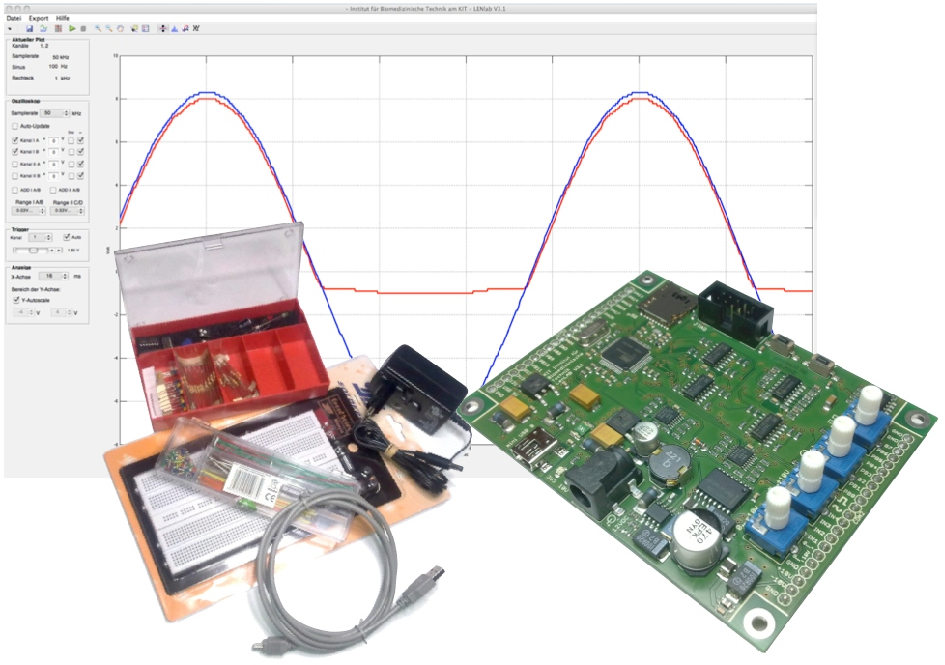
\includegraphics[width=8cm]{etit_titelbild}
    \caption{Die Materialien der Projektarbeit.}
    \label{fig:materialien}
\end{figure}
\end{verbatim}

Mit dem \verb|\ref|-Befehl lässt sich im Fließtext auf Abbildungen verweisen, z. B. verweist \verb|\ref{fig:materialien}| auf die Workshopmaterialen in Abbildung \ref{fig:materialien}, wo zuvor mit dem \verb|\label|-Befehl die Kennung \verb|fig:materialien| definiert wurde.

\begin{figure}[htb]
    \centering
    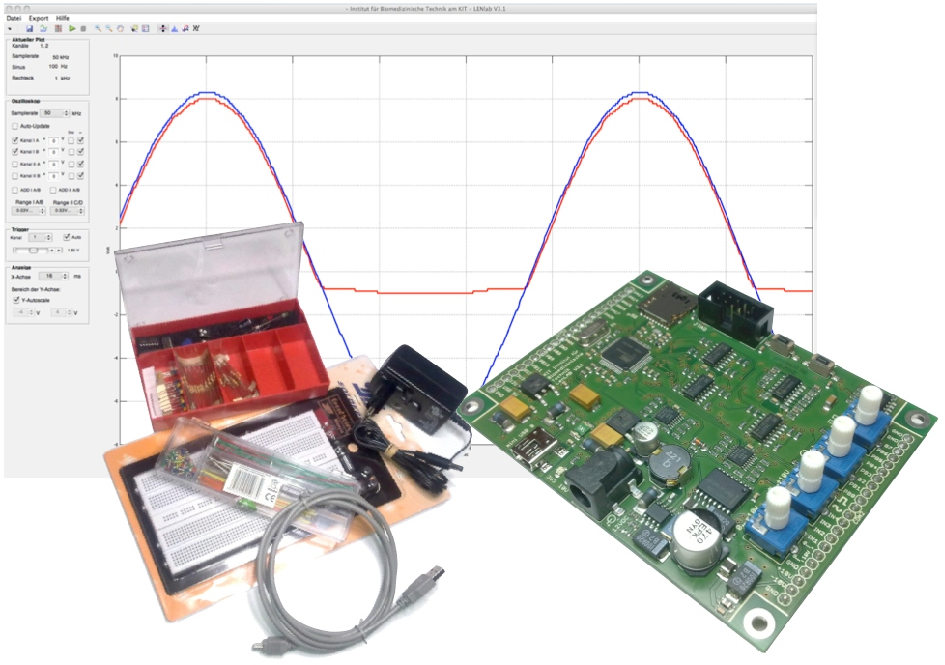
\includegraphics[width=8cm]{etit_titelbild}
    \caption{Die Materialien der Projektarbeit.}
    \label{fig:materialien}
\end{figure}


\subsection{Tabellen}
Eine beispielhafte Messreihe ist in Tabelle \ref{tab:messwerte} angegeben.
\begin{table}[htb]
    \centering
    \caption{Messwerte Widerstand.}
    \label{tab:messwerte}
    \begin{tabular}{ccc}
        \toprule
        Spannung [\si{\volt}] & Strom [\si{\ampere}] & Widerstand [\si{\ohm}] \\
        \midrule
        \num{10} & \num{5} & \num{2} \\
        \num{20} & \num{2} & \num{10} \\
        \bottomrule
    \end{tabular}
    
\end{table}


\subsection{Aufzählungen}
Aufzählungen werden mit der \verb|itemize|-Umgebung erzeugt.
\begin{itemize}
    \item Erster Punkt.
    \item Zweiter Punkt.
\end{itemize}


\subsection{Literatur}
Im Text wird mit dem \verb|cite|-Befehl auf Buchquellen \cite{bronstein}, Konferenzbeiträge \cite{kalman} und Internetquellen \cite{atmel} verwiesen. Auf jede Referenz im Literaturverzeichnis muss mindestens einmal im Text verwiesen werden.


\subsection{Quelltext}

Mit der \verb|lstlisting|-Umgebung kann MATLAB-Quelltext direkt in der \LaTeX-Datei eingegeben werden.

\begin{verbatim}
\begin{lstlisting}[style=matlab]
% Matlab-Logo
A = membrane; 
figure 
surf(A); 
colormap('cool');
\end{lstlisting}
\end{verbatim}

\begin{lstlisting}[style=matlab]
% Matlab-Logo
A = membrane; 
figure 
surf(A); 
colormap('cool');
\end{lstlisting}

Ein komplettes MATLAB-Skript kann mit dem Befehl
\begin{verbatim}
\lstinputlisting[style=matlab]{Beispiel.m}
\end{verbatim}
eingebunden werden. Ersetzen Sie einfach den Dateinamen \textit{Beispiel.m} durch Pfad und Namen Ihres Skripts. Die Ausgabe des Skripts stellt sich wie folgt dar.
\lstinputlisting[style=matlab,caption={Beispiel-Matlab-Code.}]{Beispiel.m}

Das kleine MATLAB-Programm \textit{Beispiel.m} zeigt außerdem die Verwendung des Befehls \textit{latex.m}. Fügen Sie dazu die Datei \textit{latex.m} in das MATLAB-Verzeichnis ein bzw. stellen Sie über \textit{Set Path} sicher, dass MATLAB den Ordner, in dem sich die Datei befindet, kennt. Mit \verb|latex(M)| können Sie dann die Matrix $M$ im Befehlsfenster von MATLAB in der Form ausgeben lassen, dass Sie sie direkt in Ihr \LaTeX-File kopieren können, wie folgendes Beispiel zeigt.
\begin{verbatim}
\begin{table}[htb]
\centering
\caption{Tabelle erzeugt mit Beispiel.m}
\label{Beispieltabelle}
\begin{tabular}{ccc}
\toprule
Zeit & $\sin$-Funktion & $\cos$-Funktion\\
\midrule

$0.00000$ & $0.00000$ & $1.0000$ \\
$1.0000$ & $0.84147$ & $0.54030$ \\
$2.0000$ & $0.90930$ & $-0.41615$ \\
$3.0000$ & $0.14112$ & $-0.98999$ \\
$4.0000$ & $-0.75680$ & $-0.65364$ \\
$5.0000$ & $-0.95892$ & $0.28366$ \\
$6.0000$ & $-0.27942$ & $0.96017$ \\

\bottomrule
\end{tabular}
\end{table}
\end{verbatim}
Die gezeigte Sequenz erzeugt dann Tabelle \ref{tab:Beispieltabelle}.
\begin{table}[htb]
    \centering
    \caption{Tabelle erzeugt mit Beispiel.m.}
    \label{tab:Beispieltabelle}
    \begin{tabular}{ccc}
        \toprule
        Zeit & $\sin$-Funktion & $\cos$-Funktion\\
        \midrule
        $0.00000$ & $0.00000$ & $1.0000$ \\
        $1.0000$ & $0.84147$ & $0.54030$ \\
        $2.0000$ & $0.90930$ & $-0.41615$ \\
        $3.0000$ & $0.14112$ & $-0.98999$ \\
        $4.0000$ & $-0.75680$ & $-0.65364$ \\
        $5.0000$ & $-0.95892$ & $0.28366$ \\
        $6.0000$ & $-0.27942$ & $0.96017$ \\
        \bottomrule
    \end{tabular}
\end{table}

Quelltext in anderen Formaten, z. B. \LaTeX- oder C-Code, kann ebenfalls mit dem Befehl \verb|\lstinputlisting| eingebunden werden.